\chapter{El detector de incendios de la simulación}
\label{cap:yolo-sim}

\begin{enpocas}
Cómo se generaron las 6000 imágenes etiquetadas, cómo se entrenó YOLO26n, qué tan bien quedó y cómo
funciona el nodo que detecta fuego y humo durante el vuelo.
\end{enpocas}

\section{Por qué ajustar un modelo}

YOLO26 es la última versión publicada de Ultralytics. Los modelos preentrenados en COCO no tienen
clases de fuego ni de humo, así que se ajustó \textbf{YOLO26n} (el más rápido de la familia,
adecuado para un dron) con imágenes del propio simulador, etiquetadas automáticamente. Las clases
son \emph{fuego} y \emph{humo}.

\section{Captura del dataset}

\cod{scripts/capturar_dataset.py} abre el mundo sin dron, con una cámara de la misma óptica que la
del dron (640$\times$480, HFOV 1.3~rad), y repite: mueve el foco y la cámara a posiciones al azar,
toma una imagen y la etiqueta. Para etiquetar proyecta con el modelo de cámara estenopeica una
nube de puntos del volumen de las llamas y de la columna de humo; descarta los puntos que tapan las
copas de los árboles (y, en el mundo grande, el relieve), así que cada caja cubre solo la parte
visible.

\begin{lstlisting}[style=bash]
# Mundo 'bosque'
python3 scripts/capturar_dataset.py preparar /tmp/datos/bosque.sdf /tmp/cuadrirotor_sim_$UID/modelos
GZ_SIM_RESOURCE_PATH=/tmp/datos/modelos_captura:$PWD/models \
    gz sim -s -r --headless-rendering /tmp/datos/bosque.sdf &
python3 scripts/capturar_dataset.py capturar ~/datasets/incendio_bosque 3000

# Mundo 'bosque_grande' (relieve, rocas, animales, cielo y penacho alto)
python3 scripts/capturar_dataset.py preparar /tmp/datos/bg.sdf /tmp/cuadrirotor_sim_$UID/modelos bosque_grande
python3 scripts/capturar_dataset.py capturar ~/datasets/incendio_bosque_grande 3000 bosque_grande
\end{lstlisting}

En el mundo grande el foco se pone en cualquier punto del valle (se espera 30~s cada vez que se
mueve para que el humo se forme), y una de cada cinco tomas apunta a una roca o a un animal: son
ejemplos de lo que \emph{no} es fuego. Se capturaron 3000 imágenes en cada mundo; en el grande, 989
con fuego, 2111 con humo y 836 vacías.

\begin{leccion}
Con el primer modelo, entrenado solo con el bosque plano, una roca oscura de 2.6~m en
$(-129,-154)$ del mundo grande se detectaba como \emph{fuego}: se parece al suelo quemado del foco.
Se resolvió capturando el segundo dataset, con tomas dirigidas a rocas y animales, y reentrenando
con los dos juntos.
\end{leccion}

\section{Entrenamiento}

\begin{lstlisting}[style=bash]
~/.venvs/yolo/bin/python scripts/entrenar_yolo.py ~/datasets/incendio_bosque \
    ~/datasets/incendio_bosque_grande 60
\end{lstlisting}

El script combina los datasets (escribe \cod{~/datasets/combinado_.../data.yaml}), ajusta YOLO26n
partiendo de los pesos de COCO (60 épocas, lote de 32, imágenes de 640) en la GPU y copia el mejor
modelo a \cod{yolo/incendio_yolo26n.pt}. Resultado en el conjunto de validación: precisión 0.971,
\emph{recall} 0.946, \textbf{mAP50 = 0.988} y mAP50-95 = 0.881.

\begin{figure}[H]
\centering
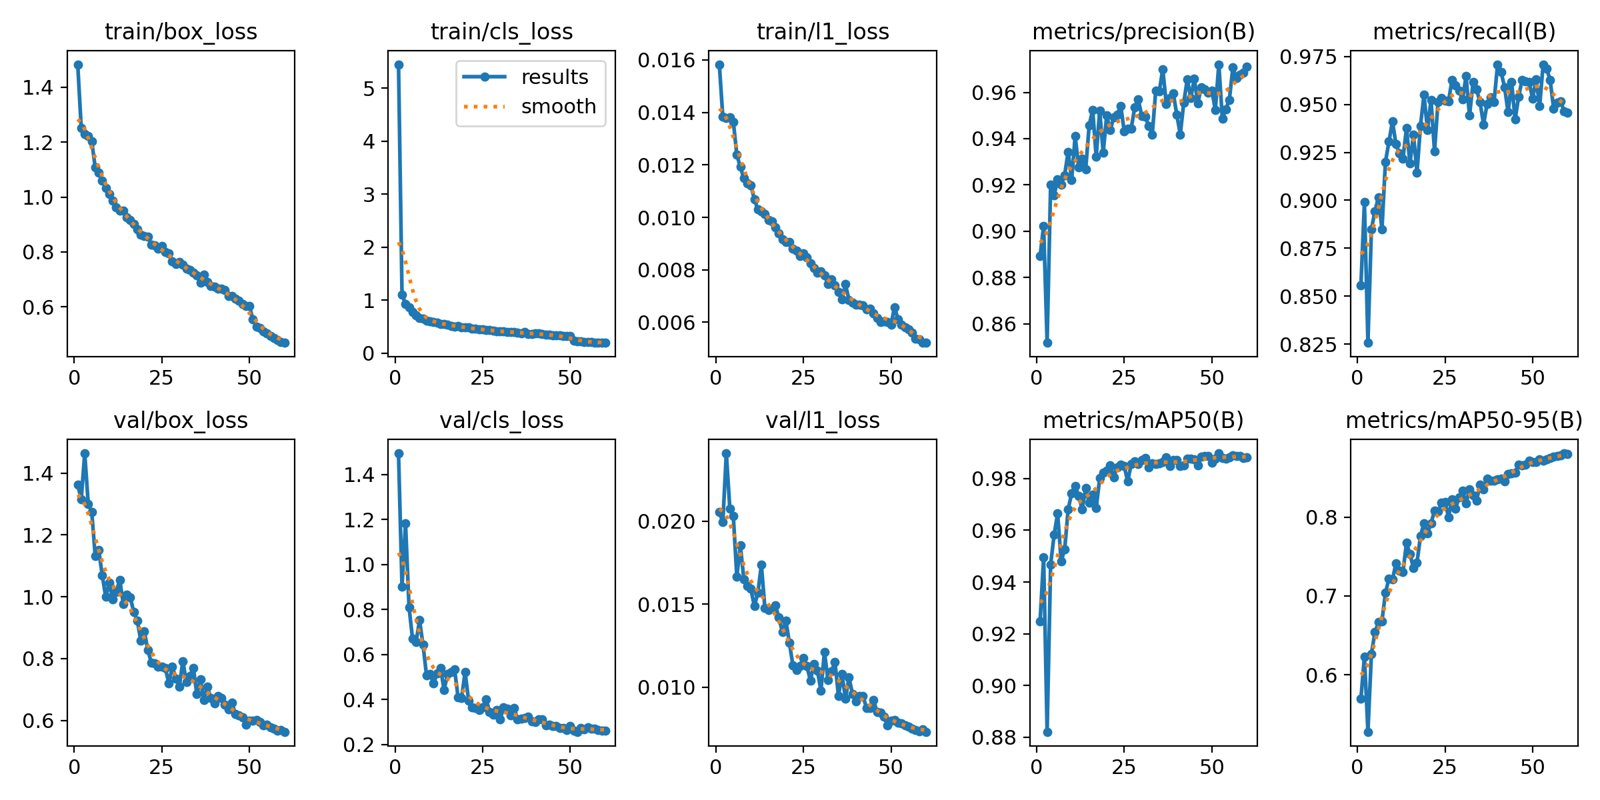
\includegraphics[width=\textwidth]{yolo_resultados.jpg}
\caption{Curvas de entrenamiento (pérdidas y métricas por época).}
\end{figure}

\begin{figure}[H]
\centering
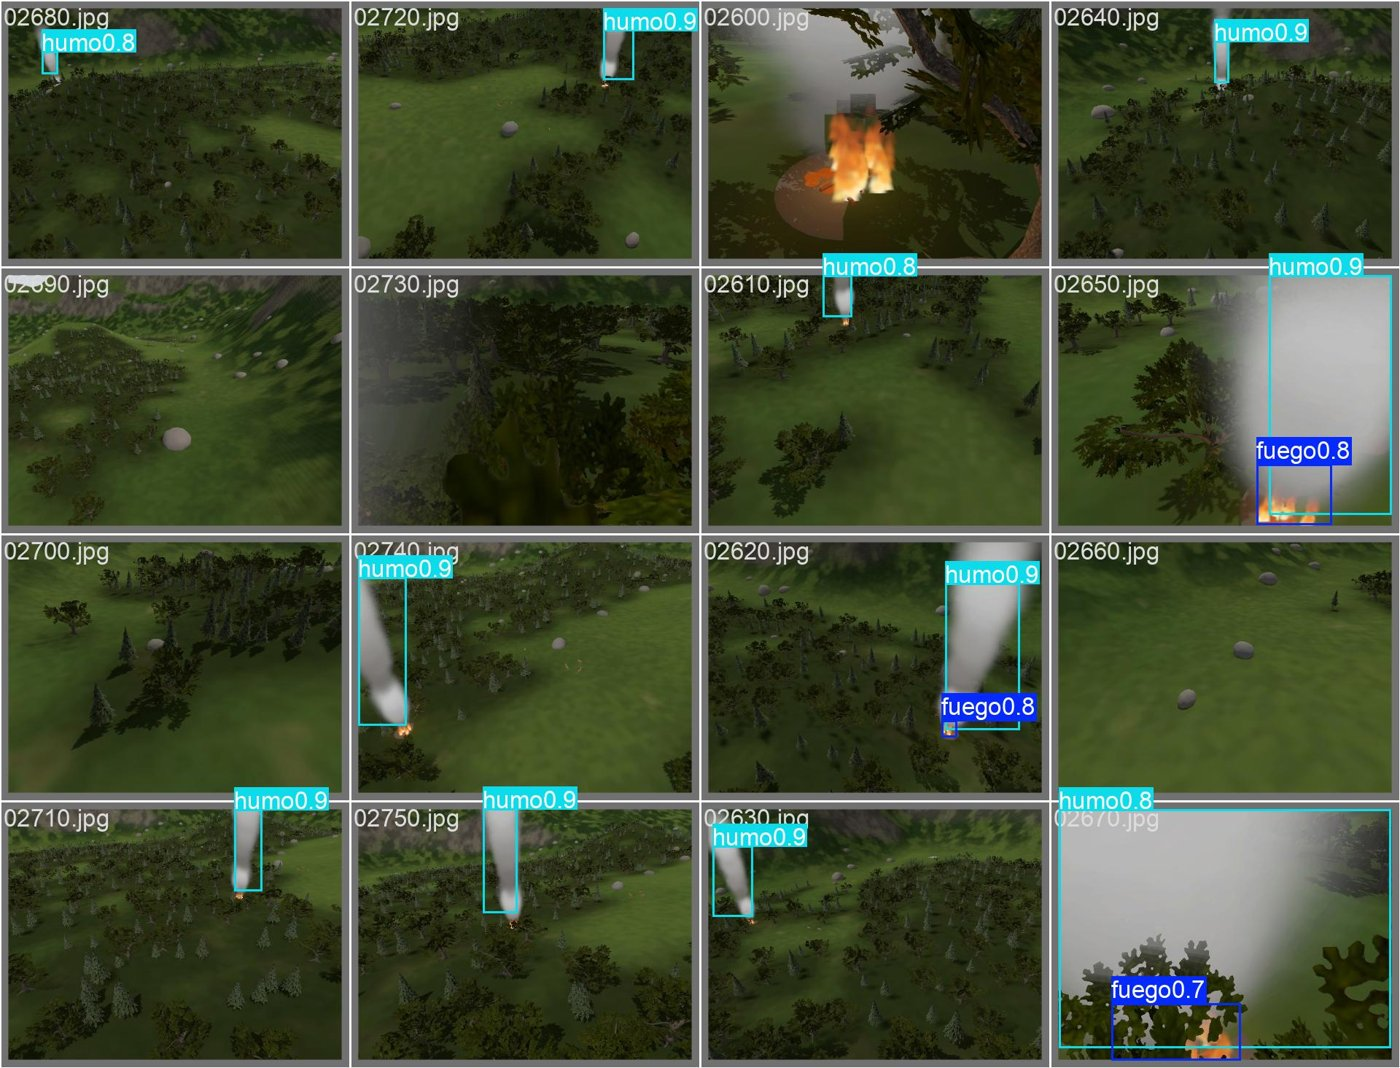
\includegraphics[width=0.8\textwidth]{yolo_val_pred.jpg}
\caption{Predicciones sobre imágenes de validación.}
\end{figure}

\begin{figure}[H]
\centering
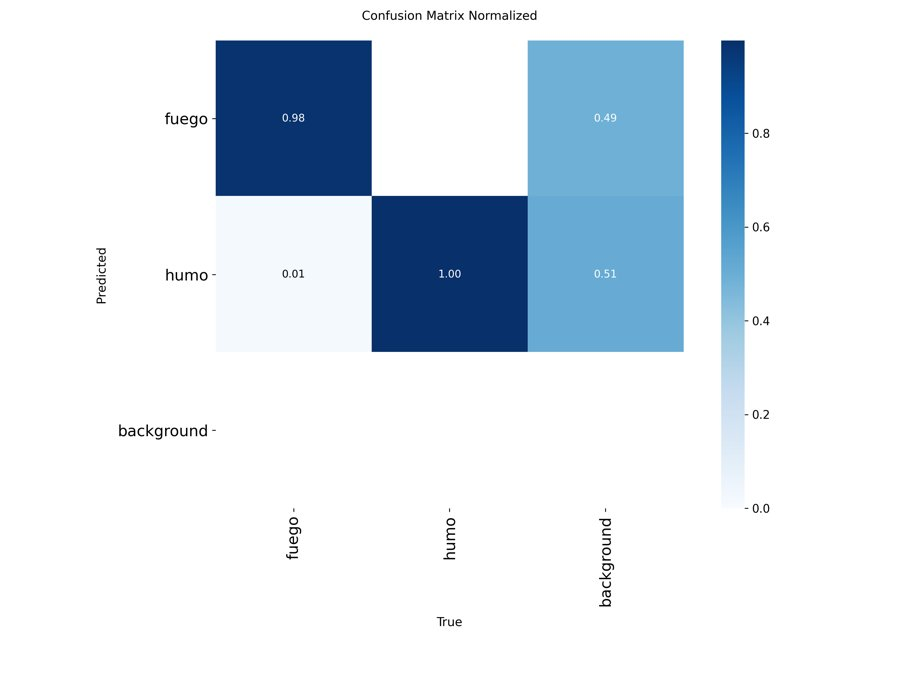
\includegraphics[width=0.55\textwidth]{yolo_confusion.jpg}
\caption{Matriz de confusión normalizada.}
\end{figure}

\section{El nodo detector}

\cod{detector_yolo.py} corre con el Python de \cod{~/.venvs/yolo}. Lee \cod{/cuadrirotor/camara},
corre el modelo en la GPU a $\approx$10~Hz y publica:
\begin{itemize}
  \item \cod{/cuadrirotor/detecciones} (\cod{vision_msgs/Detection2DArray}) con la marca de tiempo
        de la imagen, para emparejarla con la pose del dron en ese instante;
  \item \cod{/cuadrirotor/camara_yolo}: la imagen con las cajas dibujadas, que se ve en el panel
        ``Detección YOLO'' de Gazebo (\cod{config/gazebo_gui_yolo.config}).
\end{itemize}

\begin{figure}[H]
\centering
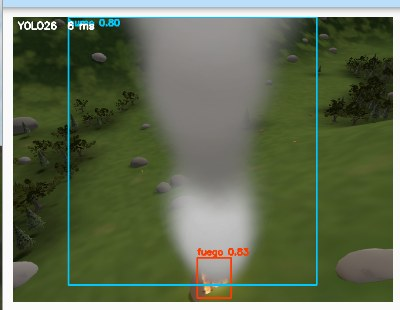
\includegraphics[width=0.5\textwidth]{yolo_panel.jpg}
\caption{Panel ``Detección YOLO'' durante la órbita: caja de \emph{humo} (cian) y de \emph{fuego}
(rojo) con su confianza.}
\end{figure}

\begin{nota}
Para volar con el dron real conviene volver a entrenar mezclando imágenes reales de incendios
(por ejemplo, el dataset D-Fire) con las del simulador.
\end{nota}
